\documentclass[a4paper,10pt]{article}

\usepackage[brazilian]{babel}
\usepackage[left=2.5cm,right=2.5cm,top=3cm,bottom=2.5cm]{geometry}
\usepackage{mathtools}
\usepackage{amsthm}
\usepackage{amsmath}
%\usepackage{nccmath}
\usepackage{amssymb}
\usepackage{amsfonts}
\usepackage{physics}
%\usepackage{dsfont}
%\usepackage{mathrsfs}

\usepackage{titling}
\usepackage{indentfirst}

\usepackage{bm}
\usepackage[dvipsnames]{xcolor}
\usepackage{cancel}

\usepackage{xurl}
\usepackage[colorlinks=true]{hyperref}

\usepackage{float}
\usepackage{graphicx}
%\usepackage{tikz}
\usepackage{caption}
\usepackage{subcaption}

%%%%%%%%%%%%%%%%%%%%%%%%%%%%%%%%%%%%%%%%%%%%%%%%%%%

\newcommand{\eps}{\epsilon}
\newcommand{\vphi}{\varphi}
\newcommand{\cte}{\text{cte}}

\newcommand{\N}{\mathbb{N}}
\newcommand{\Z}{\mathbb{Z}}
\newcommand{\Q}{\mathbb{Q}}
\newcommand{\R}{\vb{R}}
\newcommand{\C}{\mathbb{C}}
\renewcommand{\S}{\hat{S}}
%\renewcommand{\H}{\s{H}}

\renewcommand{\a}{\vb{a}}
\newcommand{\nn}{\hat{n}}
\renewcommand{\d}{\dagger}
\newcommand{\up}{\uparrow}
\newcommand{\down}{\downarrow}

\newcommand{\0}{\vb{0}}
%\newcommand{\1}{\mathds{1}}
\newcommand{\E}{\vb{E}}
\newcommand{\B}{\vb{B}}
\renewcommand{\v}{\vb{v}}
\renewcommand{\r}{\vb{r}}
\renewcommand{\k}{\vb{k}}
\newcommand{\p}{\vb{p}}
\newcommand{\q}{\vb{q}}
\newcommand{\F}{\vb{F}}

\newcommand{\s}{\sigma}
%\newcommand{\prodint}[2]{\left\langle #1 , #2 \right\rangle}
\newcommand{\cc}[1]{\overline{#1}}
\newcommand{\Eval}[3]{\eval{\left( #1 \right)}_{#2}^{#3}}

\newcommand{\unit}[1]{\; \mathrm{#1}}

\newcommand{\n}{\medskip}
\newcommand{\e}{\quad \mathrm{e} \quad}
\newcommand{\ou}{\quad \mathrm{ou} \quad}
\newcommand{\virg}{\, , \;}
\newcommand{\ptodo}{\forall \,}
\renewcommand{\implies}{\; \Rightarrow \;}
%\newcommand{\eqname}[1]{\tag*{#1}} % Tag equation with name

\setlength{\droptitle}{-7em}

\theoremstyle{plain}
\newtheorem{theorem}{Teorema}[section]
%\newtheorem{defi}[theorem]{Definição}
\newtheorem{lemma}[theorem]{Lema}
%\newtheorem{corol}[theorem]{Corolário}
%\newtheorem{prop}[theorem]{Proposição}
%\newtheorem{example}{Exemplo}
%
%\newtheorem{inneraxiom}{Axioma}
%\newenvironment{axioma}[1]
%  {\renewcommand\theinneraxiom{#1}\inneraxiom}
%  {\endinneraxiom}
%
%\newtheorem{innerpostulado}{Postulado}
%\newenvironment{postulado}[1]
%  {\renewcommand\theinnerpostulado{#1}\innerpostulado}
%  {\endinnerpostulado}
%
%\newtheorem{innerexercise}{Exercício}
%\newenvironment{exercise}[1]
%  {\renewcommand\theinnerexercise{#1}\innerexercise}
%  {\endinnerexercise}
%
%\newtheorem{innerthm}{Teorema}
%\newenvironment{teorema}[1]
%  {\renewcommand\theinnerthm{#1}\innerthm}
%  {\endinnerthm}
%
\newtheorem{innerlema}{Lema}
\newenvironment{lema}[1]
  {\renewcommand\theinnerlema{#1}\innerlema}
  {\endinnerlema}
%
%\theoremstyle{remark}
%\newtheorem*{hint}{Dica}
%\newtheorem*{notation}{Notação}
%\newtheorem*{obs}{Observação}


\title{\Huge{\textbf{Lista 5 - Mecânica Estatística}}}
\author{Mateus Marques}

\begin{document}

\maketitle

\section*{1) Paredes de domínio}

(a) Na teoria de Ginzburg-Landau para Ising, a energia livre é escrita (em dimensão $d=1$) como
$$
F = \int \dd[d]{\vb{x}} \qty{-\frac{c}{2} \phi(\vb{x}) \nabla^2 \phi(\vb{x}) + f[\phi(\vb{x})] - h \phi(\vb{x})} = \int \dd{x} \qty{-\frac{c}{2} \phi(x) \dv[2]{x} \phi(x) + f[\phi(x)] - h \phi(x)},
$$
onde $\phi$ faz o papel da magnetização e $f(\phi) = \frac{1}{2} r \phi^2 + u \phi^4$.

\n

Extremizando a energia livre, temos que
$$
0 = \fdv{F}{\phi} = -c \, \dv[2]{\phi}{x} + \dv{f[\phi(x)]}{\phi} - h.
$$

No limite de campo infinitesimal $h \to 0$ obtemos
$$
\boxed{ c \, \dv[2]{\phi}{x} = \dv{f[\phi(x)]}{\phi} = r \phi + 4u \phi^3. }
$$

Essa equação é análoga à segunda lei de Newton
$$
m \dv[2]{x}{t} = - \dv{V}{x},
$$
com as identificações $t \leftrightarrow x$, $x \leftrightarrow \phi$, $m \leftrightarrow c$ e $V(x) \leftrightarrow -f(\phi)$. A Figura \ref{fig:hill} mostra a colina de potencial nesta analogia.
\begin{figure}[H]
\centering
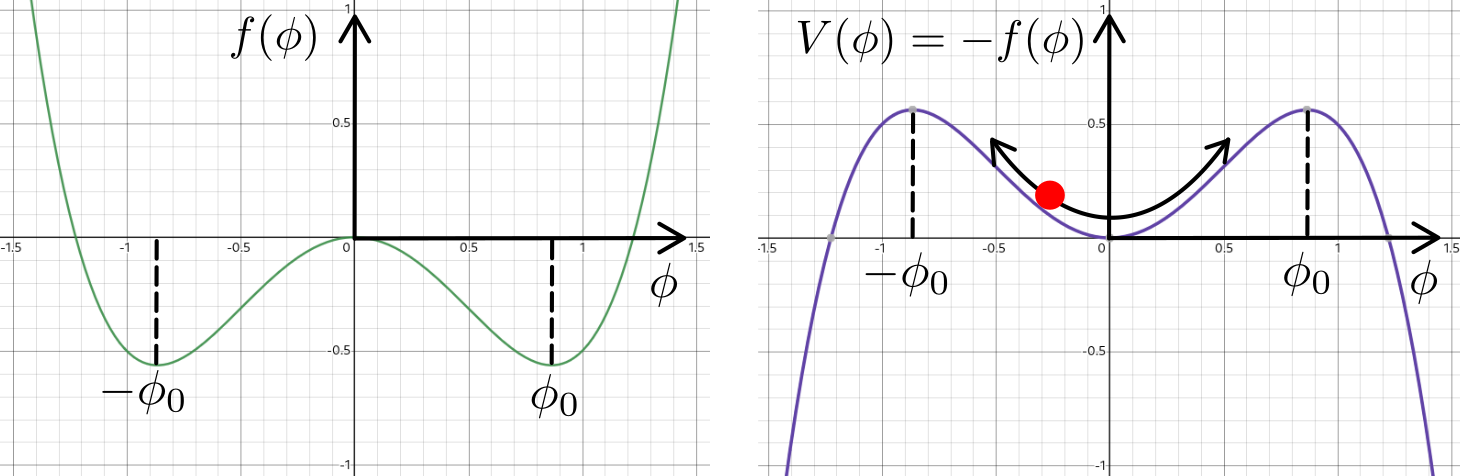
\includegraphics[width=0.9\linewidth]{fig/hill.png}
\caption{Colina de potencial $V(\phi) = -f(\phi)$.}
\label{fig:hill}
\end{figure}

\n\n

(b) Multiplicando a equação obtida por $\dd{\phi}/\dd{x}$, reconhecendo a regra da cadeia e assumindo que a energia do sistema (newtoniano) seja $E = V(\phi_0) = -f(\phi_0)$, temos
$$
\dv{x}\qty{\frac{c}{2} \qty(\dv{\phi}{x})^2 - f[\phi(x)]} = 0 \implies
\qty(\dv{\phi}{x})^2 = \frac{2}{c} \, [f(\phi) - f(\phi_0)].
$$

Lembre que $\phi_0$ é um mínimo da função $f(\phi) =  \frac{1}{2} r \phi^2 + u \phi^4$, de maneira que $\phi_0^2 = -r/4u$ e
$$
\qty(\dv{\phi}{x})^2 = \frac{2}{c} \, [f(\phi) - f(\phi_0)] = \frac{2}{c} \frac{(r + 4 u \phi^2)^2}{16 u}
= \frac{r^2}{8 \, cu} \qty(1 - \frac{\phi^2}{\phi_0^2} )^2 \implies
\boxed{ \dv{\phi}{x} = \sqrt{\frac{r^2}{8 \, cu}} \qty( 1 - \frac{\phi^2}{\phi_0^2} ). }
$$

Assumindo que $\phi(0) = 0$ (a parede de domínio está localizada em $x = 0$), temos
$$
\int_0^{\phi} \frac{\dd{\phi}}{1 - \qty(\frac{\phi^2}{\phi_0^2}) } = \sqrt{\frac{r^2}{8 \, cu}} \, \int_0^x \dd{x} \implies
\phi_0 \, \tanh[-1](\frac{\phi}{\phi_0}) = \sqrt{\frac{r^2}{8 \, cu}} \, x = \phi_0 \sqrt{\frac{-r}{2c}} \, x \implies
$$
$$
\frac{\phi}{\phi_0} = \tanh(\sqrt{\frac{-r}{2c}} \, x) \implies
\boxed{ \phi(x) = \phi_0 \tanh(\frac{x}{\sqrt{2} \, \xi}), }
$$
onde $\xi = \sqrt{-c/r}$ é o comprimento de correlação. O esboço (Figura \ref{fig:soliton}) dessa solução já foi feita na própria lista de exercícios.
\begin{figure}[H]
\centering
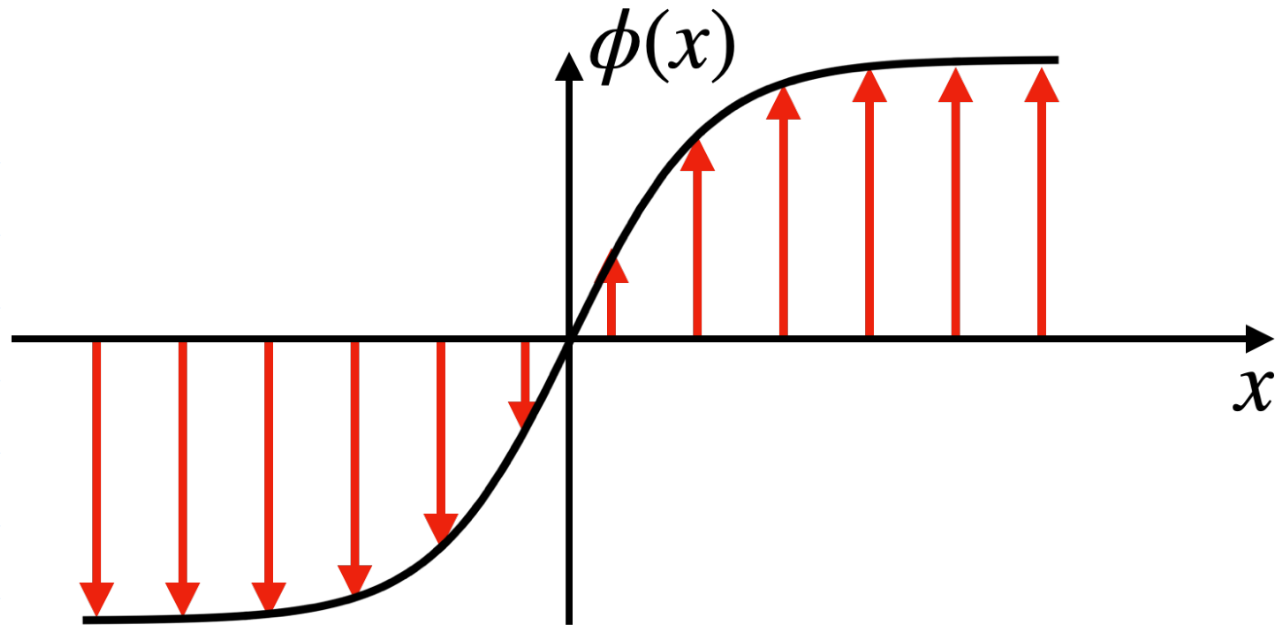
\includegraphics[width=0.6\linewidth]{fig/soliton.png}
\caption{Esboço da solução sóliton para a parede de domínio.}
\label{fig:soliton}
\end{figure}

A solução do sóliton descreve bem uma parede de domínio que leva uma distância infinita para ter os spins alinhados. Note que na localização $x = 0$ os spins mudam de direção, e eles somente se alinham totalmente em $x \to \pm \infty$, em que $\displaystyle{\lim_{x\to\pm\infty} \abs{\phi(x)} = 1}$.

\n

(c) A energia livre da solução sóliton é (lembrando que $A = \int \dd[d-1]{\vb{x}}$ é a área)
$$
F = \int \dd[d]{\vb{x}} \qty{-\frac{c}{2} \phi(\vb{x}) \nabla^2 \phi(\vb{x}) + f[\phi(\vb{x})]} =
A \int \dd{x} \qty[-\frac{c}{2} \phi \, \dv[2]{\phi}{x} + f(\phi)] =
$$
$$
= A \int \dd{x} \qty[-\frac{1}{2} \phi \, \qty(r\phi + 4u \phi^3) + \frac{r}{2} \phi^2 + u \phi^4]
= -Au \int \dd{x} \phi^4(x).
$$

A energia livre da fase ordenada $\phi(x) = \phi_0 = \sqrt{-r/4u}$, $f(\phi_0) = -\frac{r^2}{16u} = -u \phi_0^4$, é
$$
F_0 = A \int \dd{x} \qty[-\cancelto{0}{\frac{c}{2} \phi \, \dv[2]{\phi}{x}} + f(\phi)] = A \int \dd{x} f(\phi_0) =
-A u \int \dd{x} \phi_0^4.
$$

Portanto a contribuição da parede de domínio é
$$
\boxed{\Delta F = F - F_0 = Au \int \dd{x} \Big[\phi_0^4 - \phi^4(x)\Big].}
$$

\n

(d) A tensão superficial é dada por (substituindo $y = x/\sqrt{2} \xi$)
$$
\s = \frac{\Delta F}{A} = u \phi_0^4 \int_{-\infty}^{\infty} \dd{x} \qty[1 - \tanh(\frac{x}{\sqrt{2} \xi})^4] =
\sqrt{2} u \xi \phi_0^4 \int_{-\infty}^{\infty} \dd{y} \qty[1 - \tanh(y)^4].
$$

O Mathematica resolveu a integral $\int_{-\infty}^{\infty} \dd{y} \qty[1 - \tanh(y)^4] = 8/3$. Finalmente, obtemos que
$$
\boxed{\s = \frac{8\sqrt{2}}{3} \xi u \phi_0^4 = \frac{\sqrt{8}}{3} \xi u' \phi_0^4.}
$$

A tensão superficial está diferente da lista $\s' = \frac{\sqrt{8}}{3} \xi u \phi_0^4$ por um fator de $4$. Acredito que o resultado da lista dependa da definição $f'(\phi) = \frac{1}{2} r\phi^2 + \frac{u'}{4} \phi^4$, onde $\boxed{u = u'/4}$ e eu defini $f(\phi) = \frac{1}{2} r\phi^2 + u \phi^4$.


\pagebreak


\section*{4) Grupo de renomalização em uma dimensão}

(a) Considerando o sítio $S_1$, que é conectado aos sítios 0 e 2, temos para os parâmetros renormalizados $K$ e $F$
$$
e^{K'S_0 S_2 + F} = \sum_{S_1 = \pm 1} e^{K S_1(S_0 + S_2)} = e^{K(S_0+S_2)} + e^{-K(S_0+S_2)}.
$$

Como a igualdade acima deve valer para quaisquer spins $S_0 = \pm 1$ e $S_2 = \pm 1$, temos para $S_0 = S_1 = 1$ que
$$
e^{K'} e^{F} = e^{2K} + e^{-2K} = 2 \cosh(2K),
$$
e para $S_0 = 1$ e $S_2 = -1$
$$
e^{-K'} e^{F} = e^0 + e^0 = 2.
$$

Portanto:
$$
\boxed{ e^{2K'} = (e^{K'}e^{F}) (e^{K'}e^{-F}) = 2 \cosh(2K) \cdot \frac{1}{2} = \cosh(2K), }
$$
$$
e^{2F} =  (e^{K'}e^{F}) (e^{-K'}e^{F}) = 2 \cosh(2K) \cdot 2 = 4 \cosh(2K).
$$

Esse argumento não vale apenas para o sítio $S_1$, ele é geral. Podemos ver isso removendo os sítios ímpares e estudando a função de partição:
$$
Z(K) =
$$
$$
= \sum_{S_j = \pm 1} e^{K \sum_{j=-\infty}^{\infty} S_j S_{j+1}}
= \sum_{S_{2j} = \pm 1} \sum_{S_{2j + 1} = \pm 1}
\Big[
\cdots
\Big( e^{K S_{2j-2} S_{2j-1} + S_{2j-1} S_{2j}} \Big)
\Big( e^{K S_{2j} S_{2j+1} + S_{2j+1} S_{2j+2}} \Big)
\cdots
\Big]
$$
$$
= \sum_{S_{2j} = \pm 1}
\qty{
\cdots
\qty[ \sum_{S_{2j-1} = \pm 1} e^{K S_{2j-2} S_{2j-1} + S_{2j-1} S_{2j}} ]
\qty[ \sum_{S_{2j+1} = \pm 1} e^{K S_{2j} S_{2j+1} + S_{2j+1} S_{2j+2}} ]
\cdots
}
$$
$$
= \sum_{S_{2j} = \pm 1}
\qty{
\cdots
\qty[ \sum_{S_{2j-1} = \pm 1} e^{K S_{2j-1} (S_{2j-2} + S_{2j})} ]
\qty[ \sum_{S_{2j+1} = \pm 1} e^{K S_{2j+1} (S_{2j} + S_{2j+2})} ]
\cdots
}
$$
$$
= \sum_{S_{2j} = \pm 1}
\qty{
\cdots
\Big[e^{K'S_{2j-2} S_{2j} + F}\Big]
\Big[e^{K'S_{2j} S_{2j+2} + F}\Big]
\cdots
}
$$
$$
= \sum_{S_{2j} = \pm 1} \exp\qty{ \sum_{j=-\infty}^{j=\infty} \Big[K' S_{2(j-1)}S_{2j} + F\Big] }.
$$

Isso mostra que a renormalização dos parâmetros $K'$ e $F$ não depende do sítio.

\n\n

Usando a equação $2 e^{2K'} = e^{2K} + e^{-2K}$, temos
$$
\tanh^2 K = \frac{(e^K - e^{-K})^2}{(e^K + e^{-K})^2} = \frac{e^{2K} + e^{-2K} - 2}{e^{2K} + e^{-2K} + 2} =
\frac{2e^{2K'} - 2}{2e^{2K'} + 2} = \frac{e^{K'} - e^{-K'}}{e^{K'} + e^{-K'}} = \tanh(K'),
$$
o que mostra que a equação para $K'$ pode ser escrita como
$$
\boxed{ \tanh(K') = \tanh^2 K. }
$$

\n

Nas notas de aula vimos que o comprimento de correlação $\xi(K)$ é definido
$$
\xi(K) = \frac{-1}{\log(\tanh K)}.
$$

\n

Quando retiramos metade dos sítios, temos que
$$
\xi(K') = \frac{-1}{\log(\tanh K')} = \frac{-1}{\log(\tanh^2 K)} = \frac{-1}{2 \log(\tanh K)} = \frac{1}{2} \, \xi(K).
$$

\n\n

(b) Os pontos fixos $K^*$ são determinados por
$$
\tanh^2 K^* = \tanh K^* \implies \tanh K^* (\tanh K^* - 1) = 0 \implies \boxed{ K^* = 0 \ou K^* = +\infty.}
$$

\n

Lembrando que $K = \beta J$, o ponto $K^* = 0$ corresponde a $T \to +\infty$ e $K^* = +\infty$ corresponde a $T = 0$.

\n

Analisaremos a estabilidade dos dois pontos $K = 0$ e $K = +\infty$:

\n

Note que, para $K$ finito, $\tanh(K)$ tem módulo menor que 1. Assim, pela equação $\tanh(K') = \tanh^2 K$, a cada etapa de renormalização $\tanh(K)$ vai diminuindo seu módulo. No limite do infinito, teremos que $\tanh(K) \to 0 \implies K \to 0$. Isso mostra que o ponto $K = 0$ é estável, pois a renormalização iterativa faz $K \to 0$. Isso também mostra que o ponto $K = +\infty$ é instável, pois para qualquer $K$ finito a renormalização fará $K$ tender a zero, se afastando sempre do ponto $K = +\infty$.

\n

Fisicamente, a renormalização fazer $K \to 0$ nos mostra que, para qualquer $T > 0$, para flutuações de longa distância o sistema se comporta como $K$ fosse igual a zero, ou seja, como se a temperatura fosse infinita e que o sistema está na fase paramagnética (como sabemos pela solução exata em uma dimensão). Agora, para $K = +\infty$ isso mostra que a fase ferromagnética trivial em $T = 0$ (que é a temperatura crítica do modelo de Ising em 1D) é destruída para qualquer $T > 0$, ou seja, é instável.




\pagebreak

\section*{6) Modelo de Ising em um campo transverso}

(a) Este modelo é verdadeiramente quântico pois ele trata os spins como operadores quânticos (representados pelas matrizes de Pauli), diferentemente do modelo de Ising usual que os trata como variáveis binárias $\pm 1$.

\n

Considerando $T = 0$ e olhando a hamiltoniana em 1D
$$
H = -J \sum_{j} \s_j^x \s_{j+1}^x - h \sum_{j} \s_j^z,
$$
podemos imaginar o que acontece nos limites $h/J \gg 1$ e $h/J \ll 1$:
\begin{itemize}
\item $h / J \gg 1$: Neste limite só a direção $z$ importa e temos um ground-state ferromagnético $\ket{\up\up\up\cdots}$.

\item $h / J \ll 1$: Neste limite só a direção $x$ importa. O ground-state é degenerado, podendo ser combinações lineares de $\ket{\rightarrow\rightarrow\rightarrow\cdots}$ e $\ket{\leftarrow\leftarrow\leftarrow\cdots}$. Porém note que não há nenhuma preferência quanto ao eixo $z$. Isso define uma fase paramagnética.
\end{itemize}

As duas fases ferromagnética ($h/J \gg 1$) e paramagnética ($h/J \ll 1$) devem ser separadas por uma transição que depende do parâmetro de ordem $h/J$, o que configura uma transição de fase em $T = 0$, ou seja, implica na existência de um ponto crítico quântico.

\n

O diagrama de fase em $T = 0$ é esquematizado na Figura \ref{fig:qcp} abaixo.
\begin{figure}[H]
\centering
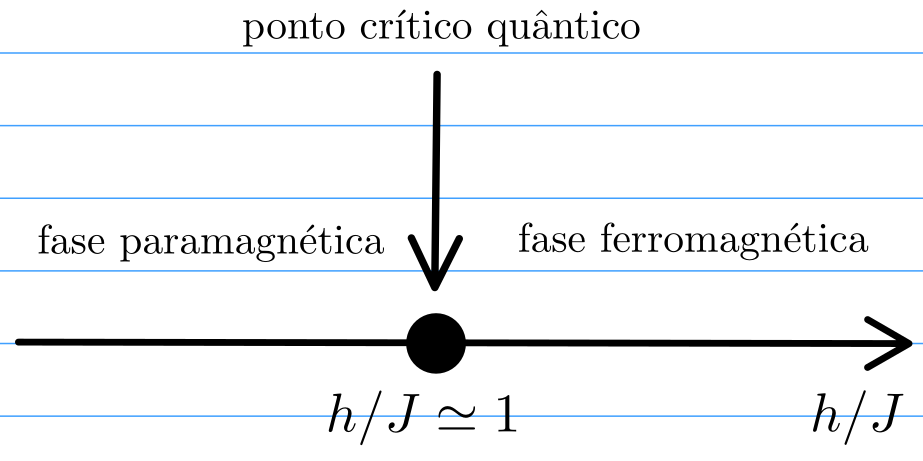
\includegraphics[width=0.8\linewidth]{fig/qcp.png}
\caption{Diagrama de fase com transição de fase quântica em $T=0$.}
\label{fig:qcp}
\end{figure}


\n\n\n\n\n\n\n\n\n\n\n

\textbf{DA LISTA DE ESTADO SOLIDO 2}

(a) Considerando $T = 0$ e olhando a hamiltoniana
$$
H = -J \sum_{j} \s_j^x \s_{j+1}^x - h \sum_{j} \s_j^z,
$$
podemos imaginar o que acontece nos limites $h/J \gg 1$ e $h/J \ll 1$:
\begin{itemize}
\item $h / J \gg 1$: Neste limite só a direção $z$ importa e temos um ground-state ferromagnético $\ket{\up\up\up\cdots}$.

\item $h / J \ll 1$: Neste limite só a direção $x$ importa. O ground-state é degenerado, podendo ser combinações lineares de $\ket{\rightarrow\rightarrow\rightarrow\cdots}$ e $\ket{\leftarrow\leftarrow\leftarrow\cdots}$. Porém note que não há nenhuma preferência quanto ao eixo $z$. Isso define uma fase paramagnética.
\end{itemize}

O diagrama de fase em $T = 0$ é da forma
%\begin{figure}[H]
%\centering
%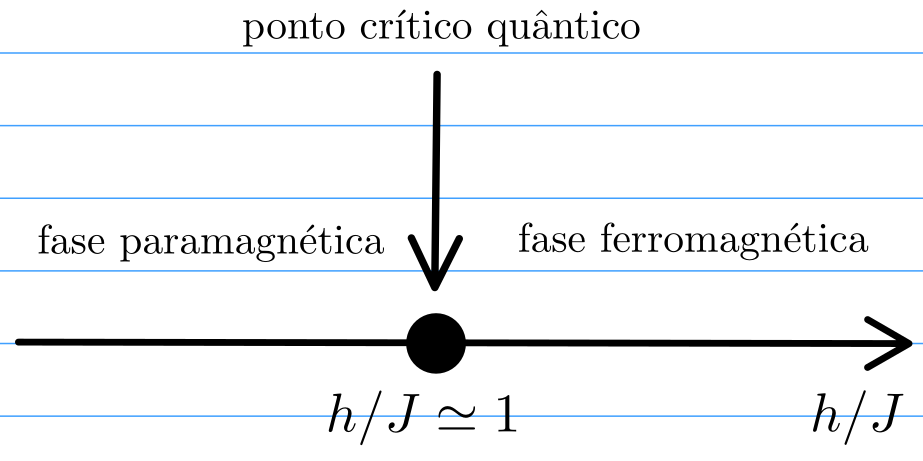
\includegraphics[width=0.75\textwidth]{fig/qcp.png}
%\caption{Diagrama de fase com transição de fase quântica em $T = 0$.}
%\label{fig:qcp}
%\end{figure}


\n

(b) Com as transformações de Jordan-Wigner
$$
\s_j^z = 1 - 2 n_j,
$$
$$
\s_j^x = \qty[\prod_{k < j} (1-2n_k)] (c_j + c_j^\d),
$$
temos que a hamiltoniana de Ising 1D em campo transverso se escreve
$$
H = -J \sum_{j} \s_j^x \s_{j+1}^x - h \sum_{j} \s_j^z =
-J \sum_{j} \qty[\prod_{k<j} (1 - 2n_k)^2] (c_j+c_j^\d)(1-2n_j)(c_{j+1} + c_{j+1}^\d) - h \sum_{j} (1-2n_j).
$$

Veja que $(1-2n_k)^2 = 1 - 4 n_k + 4 n_k^2 = 1$. Como $(c_j+c_j^\d)(1-2n_j) = c_j^\d - c_j$, temos
\begin{equation} \label{eq:hamil_transvising}
H = -J \sum_{j} \qty[ c_j^\d c_{j+1} + c_{j+1} c_j + \hc ]
+ 2h \sum_{j} c_j^\d c_j - h \sum_{j} 1.
\end{equation}

Tomando agora as transformadas $c_j = \frac{1}{\sqrt{N}} \sum_{k} e^{ikj} c_k$:
$$
H =
-\frac{J}{N} \sum_{j} \sum_{k,k'} \qty[ e^{ik'} e^{-i(k-k')j} c_k^\d c_{k'} + e^{ik'} e^{i(k+k')j} c_{k'} c_k + \hc ]
+ 2h \sum_{k} c_k^\d c_k - h N.
$$
$$
H =
-J \sum_{k} \qty[ e^{ik} c_k^\d c_{k} + e^{-ik} c_{-k} c_k + \hc ]
+ h \sum_{k} (c_k^\d c_k - c_{-k} c_{-k}^\d).
$$
$$
H =
\frac{1}{2}
\sum_{k}
\begin{pmatrix}
c_k^\d & c_{-k}
\end{pmatrix}
\begin{pmatrix}
2(h - J \cos k) & -2iJ \sin k \\
2iJ \sin k & -2(h - J\cos k)
\end{pmatrix}
\begin{pmatrix}
c_k \\ c_{-k}^\d
\end{pmatrix}
+ \cte.
$$

É imediato que os autovalores são $\omega(k) = \pm 2\sqrt{J^2 + h^2 - 2hJ \cos k}$. A transformação de Bogoliubov que diagonaliza a hamiltoniana é
$$
\begin{pmatrix}
c_k \\ c_{-k}^\d
\end{pmatrix}
=
\begin{pmatrix}
 \cos \theta_k & i\sin \theta_k  \\
i\sin \theta_k &  \cos \theta_k
\end{pmatrix}
\begin{pmatrix}
a_k \\ a_{-k}^\d
\end{pmatrix},
$$
e fazendo as contas, descobre-se que $\tan(2\theta_k) = \frac{J \sin k}{h - J \cos k}$.

%\begin{figure}[H]
%\centering
%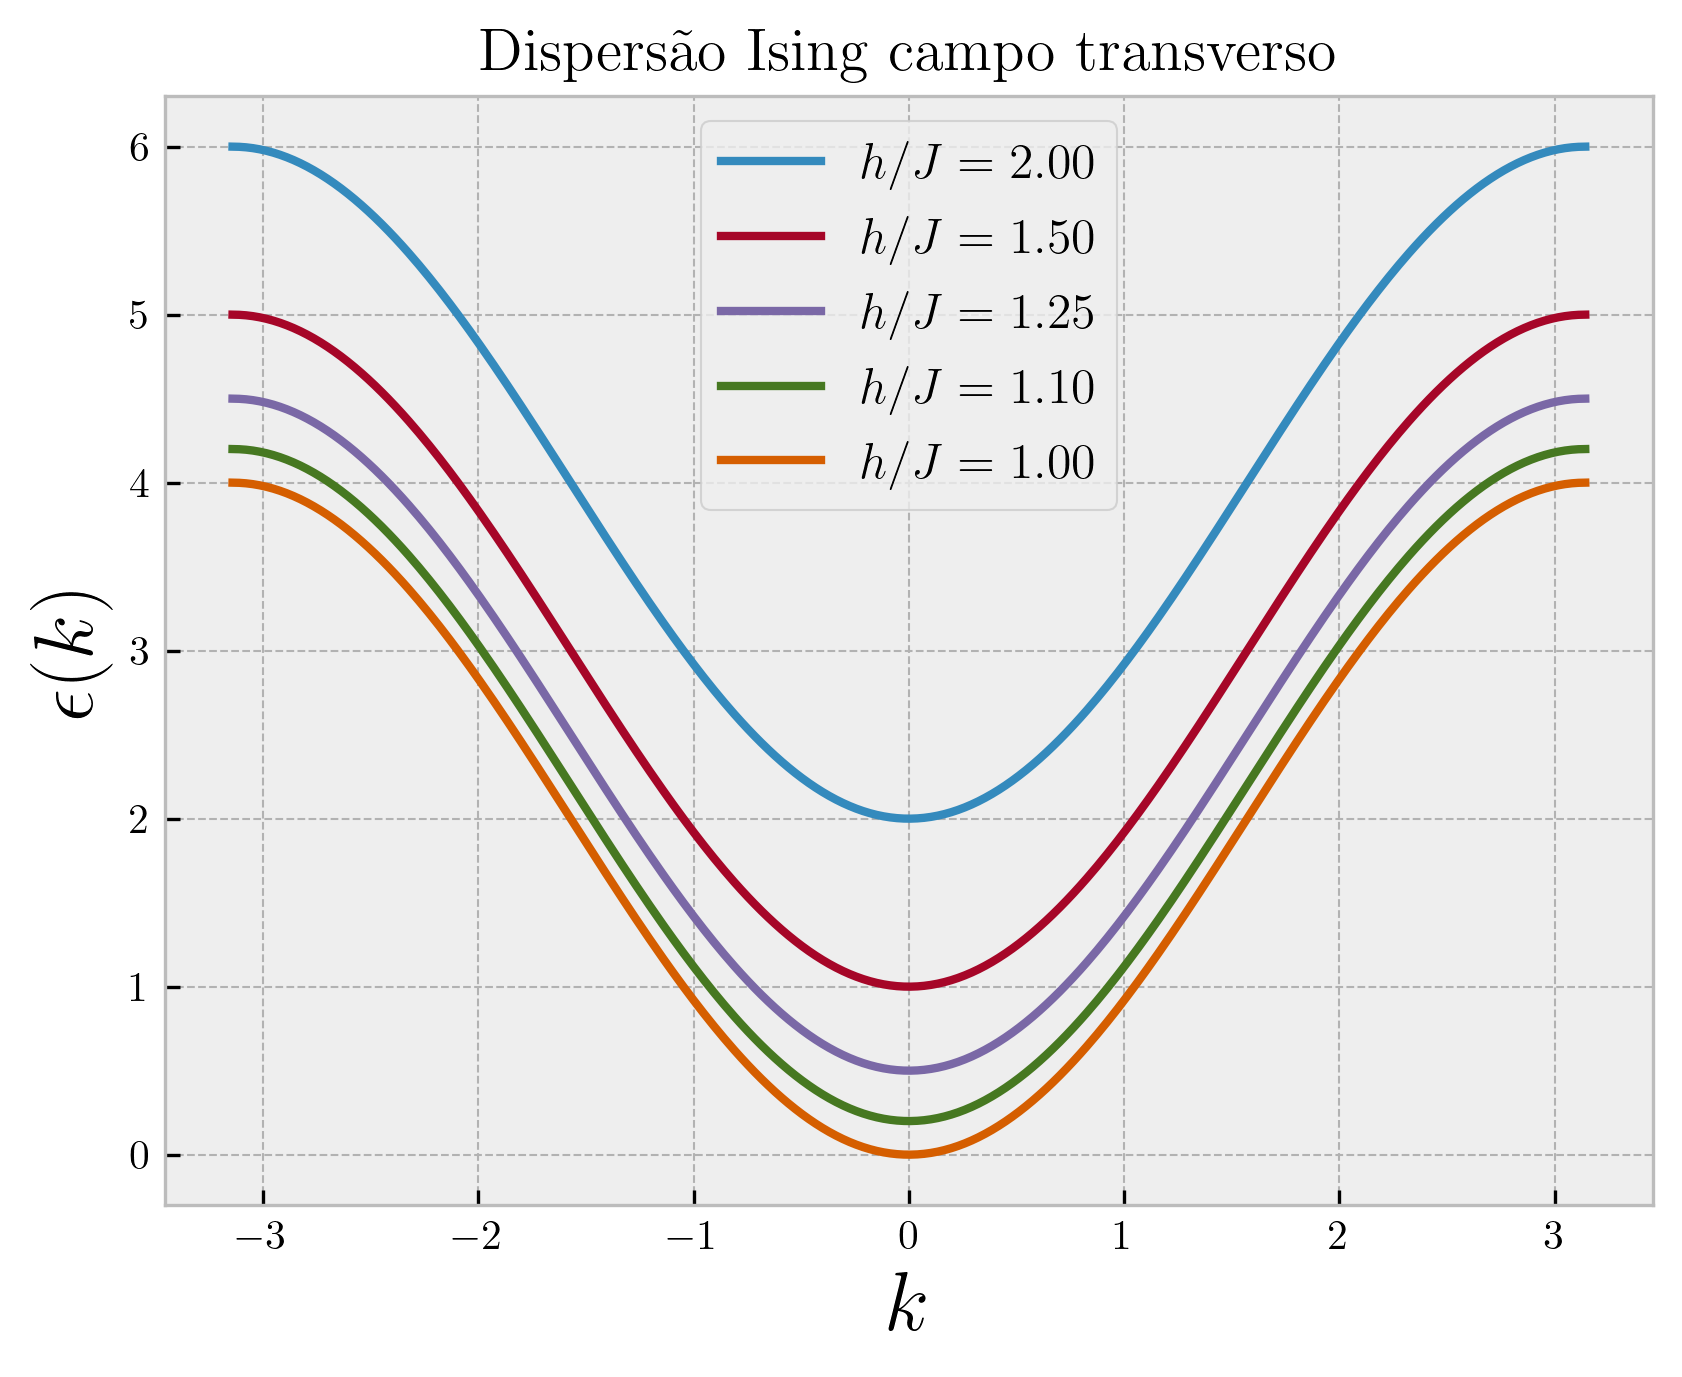
\includegraphics[width=0.5\textwidth]{fig/transv_ising.png}
%\caption{Dispersão $\omega(k) = 2\sqrt{J^2 + h^2 - 2hJ \cos k}$ para várias razões $h/J$. Vemos que para $h/J = 1$ a curva forma um cone (fecha o gap).}
%\label{fig:transv_ising}
%\end{figure}

Olhando para a Figura \ref{fig:transv_ising}, podemos identificar que a transição de fase quântica ocorre quando $h/J = 1$, que é o valor em que a dispersão forma um cone em torno de $k = 0$ (fechamento do gap).

\n

A magnetização é dada por
$$
m_z = \frac{1}{N} \sum_{j} \ev{\s_j^z} = 2 \frac{1}{N}\sum_{k} \ev{c_k^\d c_k} - 1.
$$

Pela transformação de Bogoliubov tem-se
$$
c_k^\d c_k = \cos[2](\theta_k) a_k^\d a_k + \sin[2](\theta_k) a_{-k}a_{-k}^\d
+ i \sin\theta_k \cos\theta_k (a_{k}^\d a_{-k}^\d - a_{-k} a_{-k})
$$

Para $T = 0$ temos que $\ev{X} = \ev{X}{0}$ e que $a_k \ket{0} = 0$. Portanto $\ev{c_k^\d c_k} = \sin[2](\theta_k)$. Usando que $2 \sin[2](x) = \frac{\tan[2](2x)}{1 + \tan[2](2x)}$, obtemos que
$$
m_z + 1 = \int_{-\pi}^{\pi} \frac{J^2 \sin[2](k)}{[h-J\cos(k)]^2 + J^2\sin[2](k)} \dd{k}.
$$
Pedindo para o Mathematica resolver a integral acima, ele retorna
$$
m_z + 1 =
\begin{cases}
\; \pi \frac{J^2}{h^2} , \quad h/J \geq 1, \\
\; \pi , \quad \quad \, h/J < 1. \\
\end{cases}
$$

Acho que o resultado acima não faz sentido né... Mas não sei como consertar.

\n

(d) O hamiltoniano de Kitaev é
$$
H = -t \sum_{i} (c_{i+1}^\d c_i + \hc) - \mu \sum_{i} c_i^\d c_i
+ \Delta \sum_{i} (c_{i+1}^\d c_i^\d + \hc).
$$

É fácil ver que a hamiltoniana do Ising transverso \ref{eq:hamil_transvising} é um caso particular do Kitaev para $\Delta = -J$, $t = J$ e $\mu = -2h$. Como podemos ver em \url{https://topocondmat.org/w1_topointro/1D.html}, para o modelo de Kitaev, a fase trivial acontece para $\abs{\mu} < 2t$ e a topológica para $\abs{\mu} > 2t$. Essas duas fases correspondem à paramagnética e ferromagnética do Ising transversal, respectivamente.



%%%-----
%%% Referências bibliográficas
%%%-----
%\addcontentsline{toc}{chapter}{\bibname}
%%\bibliographystyle{abntex2-num}
%\bibliography{citations}
%\bibliographystyle{ieeetr}


\end{document}
